% Options for packages loaded elsewhere
\PassOptionsToPackage{unicode}{hyperref}
\PassOptionsToPackage{hyphens}{url}
\PassOptionsToPackage{dvipsnames,svgnames,x11names}{xcolor}
%
\documentclass[
  NewProceedings,
  letterpaper]{./assets/ascelike-new}

\usepackage{amsmath,amssymb}
\usepackage{lmodern}
\usepackage{iftex}
\ifPDFTeX
  \usepackage[T1]{fontenc}
  \usepackage[utf8]{inputenc}
  \usepackage{textcomp} % provide euro and other symbols
\else % if luatex or xetex
  \usepackage{unicode-math}
  \defaultfontfeatures{Scale=MatchLowercase}
  \defaultfontfeatures[\rmfamily]{Ligatures=TeX,Scale=1}
\fi
% Use upquote if available, for straight quotes in verbatim environments
\IfFileExists{upquote.sty}{\usepackage{upquote}}{}
\IfFileExists{microtype.sty}{% use microtype if available
  \usepackage[]{microtype}
  \UseMicrotypeSet[protrusion]{basicmath} % disable protrusion for tt fonts
}{}
\usepackage{xcolor}
\setlength{\emergencystretch}{3em} % prevent overfull lines
\setcounter{secnumdepth}{-\maxdimen} % remove section numbering
% Make \paragraph and \subparagraph free-standing
\ifx\paragraph\undefined\else
  \let\oldparagraph\paragraph
  \renewcommand{\paragraph}[1]{\oldparagraph{#1}\mbox{}}
\fi
\ifx\subparagraph\undefined\else
  \let\oldsubparagraph\subparagraph
  \renewcommand{\subparagraph}[1]{\oldsubparagraph{#1}\mbox{}}
\fi


\providecommand{\tightlist}{%
  \setlength{\itemsep}{0pt}\setlength{\parskip}{0pt}}\usepackage{longtable,booktabs,array}
\usepackage{calc} % for calculating minipage widths
% Correct order of tables after \paragraph or \subparagraph
\usepackage{etoolbox}
\makeatletter
\patchcmd\longtable{\par}{\if@noskipsec\mbox{}\fi\par}{}{}
\makeatother
% Allow footnotes in longtable head/foot
\IfFileExists{footnotehyper.sty}{\usepackage{footnotehyper}}{\usepackage{footnote}}
\makesavenoteenv{longtable}
\usepackage{graphicx}
\makeatletter
\def\maxwidth{\ifdim\Gin@nat@width>\linewidth\linewidth\else\Gin@nat@width\fi}
\def\maxheight{\ifdim\Gin@nat@height>\textheight\textheight\else\Gin@nat@height\fi}
\makeatother
% Scale images if necessary, so that they will not overflow the page
% margins by default, and it is still possible to overwrite the defaults
% using explicit options in \includegraphics[width, height, ...]{}
\setkeys{Gin}{width=\maxwidth,height=\maxheight,keepaspectratio}
% Set default figure placement to htbp
\makeatletter
\def\fps@figure{htbp}
\makeatother
\newlength{\cslhangindent}
\setlength{\cslhangindent}{1.5em}
\newlength{\csllabelwidth}
\setlength{\csllabelwidth}{3em}
\newlength{\cslentryspacingunit} % times entry-spacing
\setlength{\cslentryspacingunit}{\parskip}
\newenvironment{CSLReferences}[2] % #1 hanging-ident, #2 entry spacing
 {% don't indent paragraphs
  \setlength{\parindent}{0pt}
  % turn on hanging indent if param 1 is 1
  \ifodd #1
  \let\oldpar\par
  \def\par{\hangindent=\cslhangindent\oldpar}
  \fi
  % set entry spacing
  \setlength{\parskip}{#2\cslentryspacingunit}
 }%
 {}
\usepackage{calc}
\newcommand{\CSLBlock}[1]{#1\hfill\break}
\newcommand{\CSLLeftMargin}[1]{\parbox[t]{\csllabelwidth}{#1}}
\newcommand{\CSLRightInline}[1]{\parbox[t]{\linewidth - \csllabelwidth}{#1}\break}
\newcommand{\CSLIndent}[1]{\hspace{\cslhangindent}#1}

\usepackage[labelfont=bf,labelsep=period]{caption}
\usepackage{newtxtext,newtxmath}
\makeatletter
\makeatother
\makeatletter
\@ifpackageloaded{caption}{}{\usepackage{caption}}
\AtBeginDocument{%
\ifdefined\contentsname
  \renewcommand*\contentsname{Table of contents}
\else
  \newcommand\contentsname{Table of contents}
\fi
\ifdefined\listfigurename
  \renewcommand*\listfigurename{List of Figures}
\else
  \newcommand\listfigurename{List of Figures}
\fi
\ifdefined\listtablename
  \renewcommand*\listtablename{List of Tables}
\else
  \newcommand\listtablename{List of Tables}
\fi
\ifdefined\figurename
  \renewcommand*\figurename{Fig.}
\else
  \newcommand\figurename{Fig.}
\fi
\ifdefined\tablename
  \renewcommand*\tablename{Table}
\else
  \newcommand\tablename{Table}
\fi
}
\@ifpackageloaded{float}{}{\usepackage{float}}
\floatstyle{ruled}
\@ifundefined{c@chapter}{\newfloat{codelisting}{h}{lop}}{\newfloat{codelisting}{h}{lop}[chapter]}
\floatname{codelisting}{Listing}
\newcommand*\listoflistings{\listof{codelisting}{List of Listings}}
\makeatother
\makeatletter
\@ifpackageloaded{caption}{}{\usepackage{caption}}
\@ifpackageloaded{subcaption}{}{\usepackage{subcaption}}
\makeatother
\makeatletter
\@ifpackageloaded{tcolorbox}{}{\usepackage[many]{tcolorbox}}
\makeatother
\makeatletter
\@ifundefined{shadecolor}{\definecolor{shadecolor}{rgb}{.97, .97, .97}}
\makeatother
\makeatletter
\makeatother
\ifLuaTeX
  \usepackage{selnolig}  % disable illegal ligatures
\fi
\IfFileExists{bookmark.sty}{\usepackage{bookmark}}{\usepackage{hyperref}}
\IfFileExists{xurl.sty}{\usepackage{xurl}}{} % add URL line breaks if available
\urlstyle{same} % disable monospaced font for URLs
\hypersetup{
  pdfauthor={Author One},
  colorlinks=true,
  linkcolor={blue},
  filecolor={Maroon},
  citecolor={Blue},
  urlcolor={Blue},
  pdfcreator={LaTeX via pandoc}}

\author{Author One}
\date{}

\begin{document}
\ifdefined\Shaded\renewenvironment{Shaded}{\begin{tcolorbox}[borderline west={3pt}{0pt}{shadecolor}, boxrule=0pt, sharp corners, frame hidden, breakable, interior hidden, enhanced]}{\end{tcolorbox}}\fi

\title{Template for Preparing Your Submission to the American Society Of Civil Engineers (ASCE)}

\author[2]{Author Two}
\author[3]{Author Three}

\affil[1]{First affiliation address, with corresponding author email. Email: author.one@email.com}
\affil[2]{Second affiliation address}
\affil[2]{Third affiliation address}

\maketitle

\hypertarget{abstract}{%
\section{Abstract}\label{abstract}}

The abstract should be a single paragraph (150-175 words long) written
in plain language and include a summary of the key conclusions of the
manuscript. It should clearly state the purpose of the work, the scope
of the effort, the procedures used to execute the work, and major
findings. The abstract is the second most important online search
discovery element, after the title. Authors should review the abstract
to ensure that it accurately reflects the revised paper and should
strive to include any applicable keywords that would likely be used
during an online search. Mathematics and references are not permitted in
the abstract and will be removed by the copyeditors.

\hypertarget{introduction}{%
\section{Introduction}\label{introduction}}

This template and class file ``\texttt{ascelike-new.cls}'' produce
manuscripts that comply with the guidelines of the American Society of
Civil Engineers (ASCE). It has been produced by
\href{https://www.overleaf.com}{Overleaf} in conjunction with the ASCE,
and is based on the unofficial ``\texttt{ascelike.cls}'' developed by
Matthew R.~Kuhn.

This template provides guidance on how to prepare your manuscript
according to the ASCE requirements, including details on how to use
various LaTeX commands to achieve the appropriate formatting. Additional
template options are given in Appendix \ref{sec-app-options}. If you
have any questions about this template, or need help with LaTeX, please
\href{https://www.overleaf.com/contact}{contact Overleaf} who can
provide assistance as required.

Once your work is complete, please use the ``Submit to ASCE'' option in
Overleaf to select the appropriate journal for your manuscript and
follow the instructions to complete your submission.

For more information on the ASCE, and to access additional resources for
authors, please visit the
\href{http://ascelibrary.org/page/authors}{ASCE Library website}.

\hypertarget{preparing-your-manuscript}{%
\section{Preparing Your Manuscript}\label{preparing-your-manuscript}}

\hypertarget{length}{%
\subsection{Length}\label{length}}

For most ASCE journals, the maximum length for technical papers and case
studies is 30 double-spaced manuscript pages including references,
figures, tables, and captions; 7 double-spaced manuscript pages for
technical notes; and 4 double-spaced manuscript pages for discussions
and closures. The editor may waive these restrictions to encourage
manuscripts on topics that cannot be treated within these limitations.
See the
\href{https://ascelibrary.org/doi/pdf/10.1061/9780784479018}{``Publishing
in ASCE Journals: A Guide for Authors''} for information on other
article types.

\hypertarget{general-flow-of-the-paper}{%
\subsection{General Flow of the Paper}\label{general-flow-of-the-paper}}

Sections of the article should not be numbered and use word headings
only. Article sections should appear in the following order:

\begin{itemize}
\item
  Title page content (includes title, author byline \& affiliation,
  abstract)
\item
  Introduction
\item
  Main text sections
\item
  Conclusion
\item
  Appendix(es)
\item
  Data Availability Statement
\item
  Acknowledgments
\item
  Disclaimers
\item
  Notation list
\item
  Supplemental Materials
\item
  References
\end{itemize}

\hypertarget{title}{%
\subsection{Title}\label{title}}

Titles should be no longer than 100 characters including spaces. The
title of a paper is the first ``description'' of a paper found via
search engine. Authors should take care to ensure that the title is
specific and accurately reflects the final, post-peer reviewed version
of the paper. Authors should try to include relevant search terms in the
title of the paper to maximize discoverability online. Titles should not
begin with ``A,'' ``An,'' ``The,'' ``Analysis of,'' ``Theory of,'' ``On
the,'' ``Toward,'' etc.

\hypertarget{author-bylines}{%
\subsection{Author Bylines}\label{author-bylines}}

Under the title of the manuscript, the full name of each author and his
or her affiliation and professional designation, if applicable, must be
included. The following academic and professional designations are
currently acceptable for all journals: Ph.D., Dr.Tech., Dr.Eng., D.Sc.,
Sc.D., J.D., P.E., S.E., D.WRE, Hon.D.WRE, D.GE, D.CE, D.OE, D.PE, D.NE,
NAE, DEE, P.Eng., CEng, L.S., P.L.S., G.E., P.G., P.H., RA, AICP, and
CPEng.

Former affiliations are permissible only if an author's affiliation has
changed after a manuscript has been submitted for publication. If a
coauthor has passed away, include the date of death in the affiliation
line. Any manuscript submitted without a separate affiliation statement
for each author will be returned to the corresponding author for
correction.

\hypertarget{gender-specific-words}{%
\subsection{Gender-specific Words}\label{gender-specific-words}}

Authors should avoid ``he,'' ``she,'' ``his,'' ``her,'' and ``hers.''
Alternatively, words such as ``author,'' ``discusser,'' ``engineer,''
and ``researcher'' should be used.

\hypertarget{footnotes-and-endnotes}{%
\subsection{Footnotes and Endnotes}\label{footnotes-and-endnotes}}

Footnotes and endnotes are not permitted in the text. Authors must
incorporate any necessary information within the text of the manuscript.

\textbf{Exception} - Endnotes are only permitted for use in the
\emph{Journal of Legal Affairs and Dispute Resolution in Engineering and
Construction}.

\hypertarget{si-units}{%
\subsection{SI Units}\label{si-units}}

The use of Système Internationale (SI) units as the primary units of
measure is mandatory. Other units of measurement may be given in
parentheses after the SI unit if the author desires. More information
about SI units can be found on the
\href{http://physics.nist.gov/cuu/Units/index.html}{NIST website}.

\hypertarget{conclusions}{%
\subsection{Conclusions}\label{conclusions}}

At the end of the manuscript text, authors must include a set of
conclusions, or summary and conclusion, in which the significant
implications of the information presented in the body of the text are
reviewed. Authors are encouraged to explicitly state in the conclusions
how the work presented contributes to the overall body of knowledge for
the profession.

\hypertarget{data-availability-statement}{%
\subsection{Data Availability
Statement}\label{data-availability-statement}}

When submitting a new and revised manuscript, authors are asked to
include a data availability statement containing one or more of the
following statements, with specific items listed as appropriate. Please
include one or more of the statements below, deleting those which do not
apply. This section should appear directly before the Acknowledgments
section.

\begin{itemize}
\item
  Some or all data, models, or code generated or used during the study
  are available in a repository online in accordance with funder data
  retention policies (provide full citations that include URLS or DOIs)
\item
  Some or all data, models, or code used during the study were provided
  by a third party (list items). Direct requests for these materials may
  be made to the provider as indicated in the Acknowledgements.
\item
  Some or all data, models, or code that support the findings of this
  study are available from the corresponding author upon reasonable
  request (list items).
\item
  Some or all data, models, or code generated or used during the study
  are proprietary or confidential in nature and may only be provided
  with restrictions (e.g.~anonymized data) (List items and
  restrictions).
\item
  All data, models, and code generated or used during the study appear
  in the submitted article.
\item
  No data, models, or code were generated or used during the study
  (e.g., opinion or data-less paper).
\end{itemize}

Please also see the guidelines at:
\url{https://ascelibrary.org/page/dataavailability}.

\hypertarget{acknowledgments}{%
\subsection{Acknowledgments}\label{acknowledgments}}

Acknowledgments are encouraged as a way to thank those who have
contributed to the research or project but did not merit being listed as
an author. The Acknowledgments should indicate what each person did to
contribute to the project.

Authors can include an Acknowledgments section to recognize any advisory
or financial help received. This section should appear after the
Conclusions and before the references. Authors are responsible for
ensuring that funding declarations match what was provided in the
manuscript submission system as part of the FundRef query. Discrepancies
may result in delays in publication.

\hypertarget{mathematics}{%
\subsection{Mathematics}\label{mathematics}}

All displayed equations should be numbered sequentially throughout the
entire manuscript, including Appendixes. Equations should be in the body
of a manuscript; complex equations in tables and figures are to be
avoided, and numbered equations are never permitted in figures and
tables. Here is an example of a displayed equation
(Eq.~\ref{eq-Einstein})

\begin{equation}\protect\hypertarget{eq-Einstein}{}{
E = m c^{2}
}\label{eq-Einstein}\end{equation}

Symbols should be listed alphabetically in a section called ``Notation''
at the end of the manuscript (preceding the references). See the
folliowing section for more details.

\hypertarget{notation-list}{%
\subsection{Notation List}\label{notation-list}}

Notation lists are optional; however, authors choosing to include one
should follow these guidelines:

\begin{itemize}
\item
  List all items alphabetically.
\item
  Capital letters should precede lowercase letters.
\item
  The Greek alphabet begins after the last letter of the English
  alphabet.
\item
  Non-alphabetical symbols follow the Greek alphabet.
\end{itemize}

Notation lists should always begin with the phrase, ``\emph{The
following symbols are used in this paper:}''; acronyms and abbreviations
are not permitted in the Notation list except when they are used in
equations as variables. Definitions should end with a semicolon. An
example Notation list has been included in this template; see Appendix
\ref{sec-app-notation}.

\hypertarget{appendixes}{%
\subsection{Appendixes}\label{appendixes}}

Appendixes can be used to record details and data that are of secondary
importance or are needed to support assertions in the text. The main
body of the text must contain references to all Appendixes. Any tables
or figures in Appendixes should be numbered sequentially, following the
numbering of these elements in the text. Appendixes must contain some
text, and need to be more than just figures and/or tables. Appendixes
containing forms or questionnaires should be submitted as Supplemental
Materials instead.

\hypertarget{sections-subsections-equations-etc.}{%
\section{Sections, subsections, equations,
etc.}\label{sections-subsections-equations-etc.}}

This section is included to explain and to test the formatting of
sections, subsections, subsubsections, equations, tables, and figures.

Section heading are automatically made uppercase; to include mathematics
or symbols in a section heading, you can use the
\texttt{\textbackslash{}lowercase\{\}} around the content,
e.g.~\texttt{\textbackslash{}lowercase\{\textbackslash{}boldmath\$c\^{}\{2\}\$\}}.

\hypertarget{an-example-subsection}{%
\subsection{An Example Subsection}\label{an-example-subsection}}

No automatic capitalization occurs with subsection headings; you will
need to capitalize the first letter of each word, as in ``An Example
Subsection.''

\hypertarget{an-example-subsubsection}{%
\subsubsection{An example
subsubsection}\label{an-example-subsubsection}}

No automatic capitalization occurs with subsubsections; you will need to
capitalize only the first letter of subsubsection headings.

\hypertarget{figures-and-tables}{%
\section{Figures and Tables}\label{figures-and-tables}}

This template includes two examples of figure
(Fig.~\ref{fig-fill-between}, Fig.~\ref{fig-asce-logo}) and a table
(Table~\ref{tbl-assembly}). Fig.~\ref{fig-fill-between} is a computed
figure with python. It has a caption with no more information than the
figure itself, a very poor practice indeed. A reference here
(\protect\hyperlink{ref-Stahl:2004a}{Stahl et al. 2004}).

\begin{figure}

{\centering 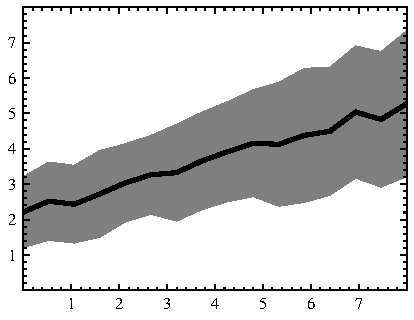
\includegraphics{example_files/figure-pdf/fig-fill-between-output-1.pdf}

}

\caption{\label{fig-fill-between}An example figure.}

\end{figure}

Fig.~\ref{fig-asce-logo} is a figure of \texttt{pdf} format.

\hypertarget{figure-captions}{%
\subsection{Figure Captions}\label{figure-captions}}

Figure captions should be short and to the point; they need not include
a complete explanation of the figure.

\hypertarget{figure-files}{%
\subsection{Figure Files}\label{figure-files}}

Figures should be uploaded as separate files in TIFF, EPS, or PDF
format. If using PDF format, authors must ensure that all fonts are
embedded before submission. Every figure must have a figure number and
be cited sequentially in the text.

\begin{figure}

{\centering 


\includegraphics{./img/asce-logo.pdf}

}

\caption{\label{fig-asce-logo}ASCE logo with signature on one line}

\end{figure}

\hypertarget{color-figures}{%
\subsection{Color Figures}\label{color-figures}}

Figures submitted in color will be published in color in the online
journal at no cost. Color figures provided must be suitable for printing
in black and white. Color figures that are ambiguous in black and white
will be returned to the author for revision, and will delay publication.
Authors wishing to have figures printed in color must indicate this in
the submission questions. There is a fee for publishing color figures in
print.

\hypertarget{table-format}{%
\subsection{Table Format}\label{table-format}}

The following is a guide to preparing tables as part of your submission

\begin{itemize}
\item
  Vertical rules should not be used in tables. Horizontal rules are used
  to offset column headings at the top of the table and footnotes (if
  any) at the bottom of the table and to separate major sections.
\item
  All columns must have a heading. Each table should have only one set
  of column headings at the top of the table. Using additional column
  headings within the body of the table should be avoided.
\item
  Photographs, sketches, line art, or other graphic elements are not
  permitted in tables. Any table that includes graphics must be treated
  and numbered as a figure.
\item
  Highlighting and shading are also not permitted and will not be
  reproduced in print. Boldface font should be used for emphasis
  sparingly.
\item
  Equations are allowed in the table body, but should be avoided if
  possible. Numbered equations are never allowed in tables.
\item
  Tables should not be submitted in multiple parts (Table 1a, 1b, etc.).
  Tables with multiple parts should either be combined into one table or
  split into separate tables.
\end{itemize}

\hypertarget{tbl-assembly}{}
\begin{longtable}[]{@{}
  >{\raggedright\arraybackslash}p{(\columnwidth - 2\tabcolsep) * \real{0.6000}}
  >{\raggedright\arraybackslash}p{(\columnwidth - 2\tabcolsep) * \real{0.4000}}@{}}
\caption{\label{tbl-assembly}An example table}\tabularnewline
\toprule()
\begin{minipage}[b]{\linewidth}\raggedright
Assembly Attribute (1)
\end{minipage} & \begin{minipage}[b]{\linewidth}\raggedright
Values (2)
\end{minipage} \\
\midrule()
\endfirsthead
\toprule()
\begin{minipage}[b]{\linewidth}\raggedright
Assembly Attribute (1)
\end{minipage} & \begin{minipage}[b]{\linewidth}\raggedright
Values (2)
\end{minipage} \\
\midrule()
\endhead
Number of particles & 4008 \\
Particle sizes & Multiple \\
Particle size range & \(0.45D_{50}^{\:\ast}\) to \(1.40D_{50}\) \\
Initial void ratio, \(e_{\mathrm{init}}\) & \(0.179\) \\
Assembly size & \(54D_{50} \times 54D_{50} \times 54D_{50}\) \\
\(\ast\) \(D_{50}\) represents the median particle diameter & \\
\bottomrule()
\end{longtable}

\hypertarget{figure-table-and-text-permissions}{%
\section{Figure, Table and Text
Permissions}\label{figure-table-and-text-permissions}}

Authors are responsible for obtaining permission for each figure,
photograph, table, map, material from a Web page, or significant amount
of text published previously or created by someone other than the
author. Permission statements must indicate permission for use online as
well as in print.

ASCE will not publish a manuscript if any text, graphic, table, or
photograph has unclear permission status. Authors are responsible for
paying any fees associated with permission to publish any material. If
the copyright holder requests a copy of the journal in which his or her
figure is used, the corresponding author is responsible for obtaining a
copy of the journal.

\hypertarget{supplemental-materials}{%
\section{Supplemental Materials}\label{supplemental-materials}}

Supplemental Materials are considered to be data too large to be
submitted comfortably for print publication (e.g., movie files, audio
files, animated .gifs, 3D rendering files) as well as color figures,
data tables, and text (e.g., Appendixes) that serve to enhance the
article, but are not considered vital to support the science presented
in the article. A complete understanding of the article does not depend
upon viewing or hearing the Supplemental Materials.

Supplemental Materials must be submitted for inclusion in the online
version of any ASCE journal via Editorial Manager at the time of
submission.

Decisions about whether to include Supplemental Materials will be made
by the relevant journal editor as part of the article acceptance
process. Supplemental Materials files will be posted online as supplied.
They will not be checked for accuracy, copyedited, typeset, or
proofread. The responsibility for scientific accuracy and file
functionality remains with the authors. A disclaimer will be displayed
to this effect with any supplemental materials published online. ASCE
does not provide technical support for the creation of supplemental
materials.

ASCE will only publish Supplemental Materials subject to full copyright
clearance. This means that if the content of the file is not original to
the author, then the author will be responsible for clearing all
permissions prior to publication. The author will be required to provide
written copies of permissions and details of the correct copyright
acknowledgment. If the content of the file is original to the author,
then it will be covered by the same Copyright Transfer Agreement as the
rest of the article.

Supplemental Materials must be briefly described in the manuscript with
direct reference to each item, such as Figure S1, Table S1, Protocol S1,
Audio S1, and Video S1 (numbering should always start at 1, since these
elements will be numbered independently from those that will appear in
the printed version of the article). Text within the supplemental
materials must follow journal style. Links to websites other than a
permanent public repository are not an acceptable alternative because
they are not permanent archives.

When an author submits supplemental materials along with a manuscript,
the author must include a section entitled ``Supplemental Materials''
within the manuscript. This section should be placed immediately before
the References section. This section should only contain a direct list
of what is included in the supplemental materials, and where those
materials can be found online. Descriptions of the supplemental
materials should not be included here. An example of appropriate text
for this section is ``Figs. S1--S22 are available online in the ASCE
Library (\href{http://ascelibrary.org/}{ascelibrary.org}).''

\hypertarget{references-citations-and-bibliographic-entries}{%
\section{References, Citations and bibliographic
entries}\label{references-citations-and-bibliographic-entries}}

ASCE uses the author-date method for in-text references, whereby the
source reads as the last names of the authors, then the year (e.g.,
Smith 2004 or Smith and Jones 2004). A References section must be
included that lists all references alphabetically by last name of the
first author.

When used together, \texttt{ascelike-new.cls} and
\texttt{ascelike-new.bst} produce citations and the References section
in the correct format automatically.

References must be published works only. Exceptions to this rule are
theses, dissertations, and ``in press'' articles, all of which are
allowed in the References list. References cited in text that are not
found in the reference list will be deleted but queried by the
copyeditor. Likewise, all references included in the References section
must be cited in the text.

The following citation options are available:

\begin{itemize}
\item
  \texttt{\textbackslash{}cite\{key\}} produces citations with full
  author list and year (\protect\hyperlink{ref-Ireland:1954a}{Ireland
  1954}).
\item
  \texttt{\textbackslash{}citeNP\{key\}} produces citations with full
  author list and year, but without enclosing parentheses: e.g.~.
\item
  \texttt{\textbackslash{}citeA\{key\}} produces citations with only the
  full author list: e.g.
\item
  \texttt{\textbackslash{}citeN\{key\}} produces citations with the full
  author list and year, but which can be used as nouns in a sentence; no
  parentheses appear around the author names, but only around the year:
  e.g.~states that \ldots{}
\item
  \texttt{\textbackslash{}citeyear\{key\}} produces the year information
  only, within parentheses, as in
  (\protect\hyperlink{ref-Ireland:1954a}{1954}).
\item
  \texttt{\textbackslash{}citeyearNP\{key\}} produces the year
  information only, as in .
\end{itemize}

The bibliographic data base \texttt{ascexmpl-new.bib} gives examples of
bibliographic entries for different document types. These entries are
from the canonical set in the ASCE web document ``Instructions For
Preparation Of Electronic Manuscripts'' and from the ASCE website. The
References section of this document has been automatically created with
the \texttt{ascelike-new.bst} style for the following entries:

\begin{itemize}
\item
  a book (\protect\hyperlink{ref-Goossens:1994a}{Goossens et al. 1994}),
\item
  an anonymous book (\protect\hyperlink{ref-Moody:1988a}{\emph{Moody's
  municipal \& government manual} 1988}),
\item
  an anonymous report using \texttt{@MANUAL}
  (\protect\hyperlink{ref-FHWA:1991a}{\emph{Evaluating scour at bridges}
  1991}),
\item
  a journal article (\protect\hyperlink{ref-Pennoni:1992a}{Pennoni
  1992}; \protect\hyperlink{ref-Stahl:2004a}{Stahl et al. 2004}),
\item
  a journal article in press
  (\protect\hyperlink{ref-Dasgupta:2008a}{Dasgupta 2008}),
\item
  an article in an edited book using \texttt{@INCOLLECTION}
  (\protect\hyperlink{ref-Zadeh:1981a}{Zadeh 1981}),
\item
  a building code using \texttt{@MANUAL}
  (\protect\hyperlink{ref-ICBO:1988a}{\emph{Uniform building code}
  1988}),
\item
  a discussion of an \texttt{@ARTICLE}
  (\protect\hyperlink{ref-Vesilind:1992a}{Vesilind 1992}),
\item
  a masters thesis using \texttt{@MASTERSTHESIS}
  (\protect\hyperlink{ref-Sotiropulos:1991a}{Sotiropulos 1991}),
\item
  a doctoral thesis using \texttt{@PHDTHESIS}
  (\protect\hyperlink{ref-Chang:1987a}{Chang 1987}),
\item
  a paper in a foreign journal
  (\protect\hyperlink{ref-Ireland:1954a}{Ireland 1954}),
\item
  a paper in a proceedings using \texttt{@INPROCEEDINGS}
  (\protect\hyperlink{ref-Eshenaur:1991a}{Eshenaur et al. 1991};
  \protect\hyperlink{ref-Garrett:2003a}{Garrett 2003}),
\item
  a standard using \texttt{@INCOLLECTION}
  (\protect\hyperlink{ref-ASTM:1991a}{ASTM 1991}),
\item
  a translated book (\protect\hyperlink{ref-Melan:1913a}{Melan 1913}),
\item
  a two-part paper (\protect\hyperlink{ref-Frater:1992a}{Frater and
  Packer 1992a}; b),
\item
  a university report using \texttt{@TECHREPORT}
  (\protect\hyperlink{ref-Duan:1990a}{Duan et al. 1990}),
\item
  an untitled item in the Federal Register using \texttt{@MANUAL}
  (\protect\hyperlink{ref-FR:1968a}{\emph{Federal register} 1988}),
\item
  works in a foreign language
  (\protect\hyperlink{ref-Duvant:1972a}{Duvant and Lions 1972};
  \protect\hyperlink{ref-Reiffenstuhl:1982a}{Reiffenstuhl 1982}),
\item
  software using \texttt{@MANUAL}
  (\protect\hyperlink{ref-Lotus:1985a}{\emph{Lotus 1-2-3 reference
  manual; release 2.01} 1985}),
\item
  two works by the same author in the same year
  (\protect\hyperlink{ref-Gaspar:2001b}{Gaspar and Koenders 2001a}; b),
  and
\item
  two works by three authors in the same year that only share the first
  two authors (\protect\hyperlink{ref-Huang2009a}{Huang et al. 2009a};
  b).
\end{itemize}

ASCE has added two types of bibliographic entries: webpages and CD-ROMs.
A webpage can be formated using the \texttt{@MISC} entry category, as
with the item (\protect\hyperlink{ref-Burka:1993a}{Burka 1993}) produced
with the following \texttt{*.bib} entry:

\begin{verbatim}
    @MISC{Burka:1993a,
      author = {Burka, L. P.},
      title = {A hypertext history of multi-user dimensions},
      journal = {MUD history},
      year = {1993},
      month = {Dec. 5, 1994},
      url = {http://www.ccs.neu.edu}
    }
\end{verbatim}

Notice the use of the ``\texttt{month}'' field to give the date that
material was downloaded and the use of a new ``\texttt{url}'' field. The
``\texttt{url}'' and \texttt{month}'' fields can also be used with other
entry types (i.e., \texttt{@BOOK}, \texttt{@INPROCEEDINGS},
\texttt{@MANUAL}, \texttt{@MASTERSTHESIS}, \texttt{@PHDTHESIS}, and
\texttt{@TECHREPORT}): for example, in the entry type
\texttt{@PHDTHESIS} for
(\protect\hyperlink{ref-Wichtmann:2005a}{Wichtmann 2005}).

A CD-ROM can be referenced when using the \texttt{@BOOK},
\texttt{@INBOOK}, \texttt{@INCOLLECTION}, or \texttt{@INPROCEEDINGS}
categories, as in the entry
(\protect\hyperlink{ref-Liggett:1998a}{Liggett and Caughey 1998}). The
field ``\texttt{howpublished}'' is used to designate the medium in the
\texttt{.bib} file:

\begin{verbatim}
    howpublished = {CD-ROM},
\end{verbatim}

\appendix

\hypertarget{sec-app-notation}{%
\section{Notation}\label{sec-app-notation}}

\emph{The following symbols are used in this paper:}

\begin{longtable}[]{@{}ll@{}}
\toprule()
\endhead
\(D\) & pile diameter (m); \\
\(R\) & distance (m); and \\
\(C_{\mathrm{Oh\;no!}}\) & fudge factor. \\
\bottomrule()
\end{longtable}

\hypertarget{sec-app-options}{%
\section{LaTeX Template Options}\label{sec-app-options}}

The document class \texttt{ascelike-new.cls} provides several options
given below. The
\texttt{Proceedings\textbar{}\textasciigrave{}\textasciigrave{}Journal\textbar{}\textasciigrave{}\textasciigrave{}NewProceedings}
option is the most important; the other options are largely incidental.

\begin{enumerate}
\def\labelenumi{\arabic{enumi}.}
\item
  Options
  \texttt{Journal\textbar{}\textasciigrave{}\textasciigrave{}Proceedings\textbar{}\textasciigrave{}\textasciigrave{}NewProceedings}
  specify the overall format of the output manuscript.

  \texttt{Journal} produces double-spaced manuscripts for ASCE journals.
  As default settings, it places tables and figures at the end of the
  manuscript and produces lists of tables and figures. It places line
  numbers within the left margin.

  \texttt{Proceedings} produces older-style camera-ready single-spaced
  manuscripts for ASCE conference proceedings. The newer ASCE style is
  enacted with the \texttt{NewProceedings} option.

  \texttt{NewProceedings} produces newer-style single-spaced manuscripts
  for ASCE conference proceedings, as shown on the ASCE website
  (\emph{ca.} 2013). As default settings, \texttt{NewProceedings} places
  figures and tables within the text. It does not place line numbers
  within the left margin.

  If desired, the bottom right corner can be ``tagged'' with the
  author's name (this can be done by inserting the command
  \texttt{\textbackslash{}NameTag\{\textless{}}\emph{your
  name}\texttt{\textgreater{}\}} within the preamble of your document).
  All of the default settings can be altered with the options that are
  described below.
\item
  Options \texttt{BackFigs\textbar{}InsideFigs} can be used to override
  the default placement of tables and figures in the \texttt{Journal},
  \texttt{Proceedings}, and \texttt{NewProceedings} formats.
\item
  Options \texttt{SingleSpace\textbar{}DoubleSpace} can be used to
  override the default text spacing in the \texttt{Journal},
  \texttt{Proceedings}, and \texttt{NewProceedings} formats.
\item
  Options \texttt{10pt\textbar{}11pt\textbar{}12pt} can be used to
  override the default text size (12pt).
\item
  The option \texttt{NoLists} suppresses inclusion of lists of tables
  and figures that would normally be included in the \texttt{Journal}
  format.
\item
  The option \texttt{NoPageNumbers} suppresses the printing of page
  numbers.
\item
  The option \texttt{SectionNumbers} produces an automatic numbering of
  sections. Without the \texttt{SectionNumbers} option, sections will
  \emph{not} be numbered, as this seems to be the usual formatting in
  ASCE journals (note that the Appendixes will, however, be
  automatically ``numbered'' with Roman numerals). With the
  \texttt{SectionNumbers} option, sections and subsections are numbered
  with Arabic numerals (e.g.~2, 2.1, etc.), but subsubsection headings
  will not be numbered.
\item
  The options \texttt{NoLineNumbers\textbar{}LineNumbers} can be used to
  override the default use (or absence) of line numbers in the
  \texttt{Journal}, \texttt{Proceedings}, and \texttt{NewProceedings}
  formats.
\end{enumerate}

\hypertarget{references}{%
\section*{References}\label{references}}
\addcontentsline{toc}{section}{References}

\hypertarget{refs}{}
\begin{CSLReferences}{1}{0}
\leavevmode\vadjust pre{\hypertarget{ref-ASTM:1991a}{}}%
ASTM. 1991. {``Standard practice for the use of the international system
of units ({ SI}) (the modernized metric system).''} \emph{E 380-91a}.
Philadelphia, Pa.: ASTM.

\leavevmode\vadjust pre{\hypertarget{ref-Burka:1993a}{}}%
Burka, L. P. 1993. {``\href{http://www.ccs.neu.edu}{A hypertext history
of multi-user dimensions}.''} \emph{MUD history}.

\leavevmode\vadjust pre{\hypertarget{ref-Chang:1987a}{}}%
Chang, T. C. 1987. {``\href{}{Network resource allocation using an
expert system with fuzzy logic reasoning}.''} PhD thesis. Berkeley, CA:
University of California.

\leavevmode\vadjust pre{\hypertarget{ref-Dasgupta:2008a}{}}%
Dasgupta, G. 2008. {``Stiffness matrix from isoparametric closed form
shape functions using exact integration.''} \emph{J. Aerosp. Eng.}

\leavevmode\vadjust pre{\hypertarget{ref-Duan:1990a}{}}%
Duan, L., J. T. Loh, and W. F. Chen. 1990. \emph{\href{}{M-{P}-f-based
analysis of dented tubular members}}. Struct. Engrg. Rep. No. West
Lafayette, Ind.: School of Civ. Engrg., Purdue Univ.

\leavevmode\vadjust pre{\hypertarget{ref-Duvant:1972a}{}}%
Duvant, G., and J. L. Lions. 1972. \emph{Les in{é}quations en
m{é}chanique et en physique}. Paris, France: Dunod.

\leavevmode\vadjust pre{\hypertarget{ref-Eshenaur:1991a}{}}%
Eshenaur, S. R., J. M. Kulicki, and D. R. Mertz. 1991. {``Retrofitting
distortion-induced fatigue cracking of non-composite steel
girder-floorbeam-stringer bridges.''} \emph{Proc., 8th annual int.
Bridge conf.}, 380--388. Pittsburgh, Pa.: Engineers' Soc. of Western
Pennsylvania.

\leavevmode\vadjust pre{\hypertarget{ref-FHWA:1991a}{}}%
\emph{Evaluating scour at bridges}. 1991. Washington, D.C.: Federal
Highway Administration (FHWA); Rep., Hydr. Engrg. Circular No. 18:
FHWA-IP-90-017.

\leavevmode\vadjust pre{\hypertarget{ref-FR:1968a}{}}%
\emph{Federal register}. 1988.

\leavevmode\vadjust pre{\hypertarget{ref-Frater:1992a}{}}%
Frater, G. S., and J. A. Packer. 1992a. {``Weldment design for {RHS}
truss connections. {I}: applications.''} \emph{J. Struct. Engrg.}, 118
(10): 2784--2803. ASCE.

\leavevmode\vadjust pre{\hypertarget{ref-Frater:1992b}{}}%
Frater, G. S., and J. A. Packer. 1992b. {``Weldment design for {RHS}
truss connections. {II}: experimentation.''} \emph{J. Struct. Engrg.},
118 (10): 2804--2820. ASCE.

\leavevmode\vadjust pre{\hypertarget{ref-Garrett:2003a}{}}%
Garrett, D. L. 2003. {``Coupled analysis of floating production
systems.''} \emph{Proc., Int. Symp. On deep mooring systems}, 152--167.
Reston, VA: ASCE; CD-ROM.

\leavevmode\vadjust pre{\hypertarget{ref-Gaspar:2001a}{}}%
Gaspar, N., and M. A. Koenders. 2001b. {``Micromechanic formulation of
macroscopic structures in a granular medium.''} \emph{J. Engrg. Mech.},
127 (10): 987--993.

\leavevmode\vadjust pre{\hypertarget{ref-Gaspar:2001b}{}}%
Gaspar, N., and M. A. Koenders. 2001a. {``Estimates of the shear modulus
of a granular assembly using heterogeneous media techniques.''}
\emph{Powders and grains 2001}, Y. Kishino, ed., 389--392. Lisse: A.A.
Balkema.

\leavevmode\vadjust pre{\hypertarget{ref-Goossens:1994a}{}}%
Goossens, M., F. Mittlebach, and A. Samarin. 1994. \emph{The
LaTeX~companion}. Reading, Mass.: Addison--Wesley Pub. Co.

\leavevmode\vadjust pre{\hypertarget{ref-Huang2009a}{}}%
Huang, Y., R. Bird, and M. Bell. 2009a. {``A comparative study of the
emission by road maintenance works and the disrupted traffic using life
cycle assessment and micro-simulation.''} \emph{Transportation Research
Part D}, 14: 197--204.

\leavevmode\vadjust pre{\hypertarget{ref-Huang2009b}{}}%
Huang, Y., R. Bird, and O. Hendrich. 2009b. {``Development of a life
cycle assessment tool for construction and maintenance of asphalt
pavements.''} \emph{Journal of Cleaner Production}, 17: 283--296.

\leavevmode\vadjust pre{\hypertarget{ref-Ireland:1954a}{}}%
Ireland, H. O. 1954. {``Stability analysis of {C}ongress {S}treet open
cut in {C}hicago.''} \emph{G{é}otechnique}, 4 (4): 163--168. London,
England.

\leavevmode\vadjust pre{\hypertarget{ref-Liggett:1998a}{}}%
Liggett, J. A., and D. A. Caughey. 1998. {``Fluid statics.''}
\emph{Fluid mechanics}, 167--177. Reston, VA: CD-ROM; ASCE.

\leavevmode\vadjust pre{\hypertarget{ref-Lotus:1985a}{}}%
\emph{Lotus 1-2-3 reference manual; release 2.01}. 1985. Cambridge,
Mass.: Lotus Development Corp.

\leavevmode\vadjust pre{\hypertarget{ref-Melan:1913a}{}}%
Melan, J. 1913. \emph{Theory of arches and suspension bridges}. Chicago,
Ill: Myron C. Clark.

\leavevmode\vadjust pre{\hypertarget{ref-Moody:1988a}{}}%
\emph{Moody's municipal \& government manual}. 1988. New York, N.Y.:
Moody's Investors Service.

\leavevmode\vadjust pre{\hypertarget{ref-Pennoni:1992a}{}}%
Pennoni, C. R. 1992. {``Visioning: The future of civil engineering.''}
\emph{J. Profl. Issues in Engrg. Education and Practice}, 118 (3):
221--233. ASCE.

\leavevmode\vadjust pre{\hypertarget{ref-Reiffenstuhl:1982a}{}}%
Reiffenstuhl, H. 1982. {``Das vorspannen von bewehrung auf druck:
Grundsaetzliches und anwendungsmoeglichkeiten {[}prestressing of
reinforcing in compression: Fundamentals and application
possibilities{]}.''} \emph{Beton-und Stahlbetonbau}, 77 (3): 69--73.
Berlin, Germany.

\leavevmode\vadjust pre{\hypertarget{ref-Sotiropulos:1991a}{}}%
Sotiropulos, S. N. 1991. {``\href{}{Static response of bridge
superstructures made of fiber reinforced plastic}.''} M.\{S\}. thesis.
Morgantown, WV: West Virginia Univ.

\leavevmode\vadjust pre{\hypertarget{ref-Stahl:2004a}{}}%
Stahl, D. C., R. W. Wolfe, and M. Begel. 2004. {``Improved analysis of
timber rivet connections.''} \emph{J. Struct. Eng.}, 130 (8):
1272--1279.

\leavevmode\vadjust pre{\hypertarget{ref-ICBO:1988a}{}}%
\emph{Uniform building code}. 1988. Whittier, Calif.: International
Conference of Building Officials.

\leavevmode\vadjust pre{\hypertarget{ref-Vesilind:1992a}{}}%
Vesilind, P. A. 1992. {``Discussion of {`{G}uidance for
engineering-design-class lectures on ethics,'} by {R}ichard {H}.
{M}c{C}uen.''} \emph{J. Profl. Issues in Engrg. Education and Practice},
118 (2): 214--215. ASCE.

\leavevmode\vadjust pre{\hypertarget{ref-Wichtmann:2005a}{}}%
Wichtmann, T. 2005.
{``\href{https://www.rz.uni-karlsruhe.de/$/sim$gn97/}{Explicit
accumulation model for non-cohesive soils under cyclic loading}.''} PhD
thesis. Institute for Soil Mechanics; Foundation Engineering, Ruhr-Univ.
Bochum, Germany.

\leavevmode\vadjust pre{\hypertarget{ref-Zadeh:1981a}{}}%
Zadeh, L. A. 1981. {``Possibility theory and soft data analysis.''}
\emph{Mathematical frontiers of the social and policy sciences}, L. Cobb
and R. M. Thrall, eds., 69--129. Boulder, Colo.: Westview Press, Inc.

\end{CSLReferences}



\end{document}
